\documentclass[../../main.tex]{subfiles}
\begin{document}

{\bf [解]}

与えられた曲線を
\begin{align}
  \begin{cases}
    x = f(t) = \cos2t \\
    y = g(t)=t\sin t
  \end{cases} \label{eq:1}
\end{align}
とおく．一階微分は
\begin{align}
  \begin{cases}
    f'(t)=-2\sin2t \\
    g'(t)=t\cos t + \sin t
  \end{cases} \label{eq:2}
\end{align}
である．従って増減表は以下のようになる．

% TODO: 増減表
\begin{table}[htb]
  \centering
  \caption{曲線 $(x, y) = (f(t), g(t))$ の増減表 $(0 \le t \le 2\pi)$}
  \label{tab:parametric_curve_monotonicity}
  \renewcommand{\arraystretch}{1.5}
  \begin{tabular}{c|c|c|c|c|c|c|c|c|c|c|c|c|c}
    \hline
    $t$ & $0$ & $\cdots$ & $\dfrac{\pi}{2}$ & $\cdots$ & $\alpha$ & $\cdots$ & $\pi$ & $\cdots$ & $\dfrac{3}{2}\pi$ & $\cdots$ & $\beta$ & $\cdots$ & $2\pi$ \\ \hline
    $f'(t)$ & $0$ & $-$ & $0$ & $+$ & $+$ & $+$ & $0$ & $-$ & $0$ & $+$ & $+$ & $+$ & $0$ \\ \hline
    $g'(t)$ & $0$ & $+$ & $+$ & $+$ & $0$ & $-$ & $-$ & $-$ & $-$ & $-$ & $0$ & $+$ & $+$ \\ \hline
    $(x, y)$ & $(1, 0)$ & $\nwarrow$ & $\left(-1, \dfrac{\pi}{2}\right)$ & $\nearrow$ & & $\searrow$ & $(1, 0)$ & $\swarrow$ & $\left(-1, -\dfrac{3}{2}\pi\right)$ & $\searrow$ & & $\nearrow$ & $(1, 0)$ \\ \hline
  \end{tabular}
  \vspace{1ex}
  \parbox{\linewidth}{\footnotesize ※ $\alpha, \beta$ はそれぞれ $0 < t < \pi$ および $\pi < t < 2\pi$ における $g'(t) = t\cos t + \sin t = 0$（すなわち $\tan t = -t$）の唯一の実数解である．}
\end{table}

ここで，$(1,0)$（$t=0,\pi,2\pi$に対応）以外にグラフの交わる点があると仮定し，対応する$t$を$t_1,t_2$とすると（$t_1\ne t_2$），$f(t_1)=f(t_2),g(t_1)=g(t_2)$だから
\begin{align}
  \begin{cases}
    \cos2t_1&=\cos2t_2 \\
    t_1\sin t_1&=t_2\sin t_2
  \end{cases} \label{eq:3}
\end{align}
である．$t<\pi$で$g(t)>0$, $t>\pi$で$g(t)<0$だから，$0<t_1<t_2<\pi$または$\pi<t_1<t_2<2\pi$で考えればよい．
\cref{eq:3}の第一式より
\begin{align}
  \begin{cases}
    2t_2=2\pi - 2t_1 & (0<t_1<t_2<\pi) \\
    2t_2=6\pi - 2t_1 & (\pi<t_1<t_2<2\pi)
  \end{cases}
  \therefore
  \begin{cases}
    t_2=\pi  - t_1 & (0<t_1<t_2<\pi) \\
    t_2=3\pi - t_1 & (\pi<t_1<t_2<2\pi)
  \end{cases} \label{eq:4}
\end{align}
であり，\cref{eq:3}の第一式に代入して
\begin{align}
  \begin{cases}
    t_1\sin t_1=(\pi-t_1)\sin t_1 & (0<t_1<t_2<\pi) \\
    t_1\sin t_1=(3\pi-t_1)\sin t_1 & (\pi<t_1<t_2<2\pi)
  \end{cases}
  \therefore
  \begin{cases}
    t_1 = \dfrac{\pi}{2} & (0<t_1<t_2<\pi) \\
    t_1 = \dfrac{3\pi}{2} & (\pi<t_1<t_2<2\pi)
  \end{cases}
\end{align}
となるが，この時どちらのケースも$t_2=t_1$となって矛盾する．
よって背理法により$(1,0)$以外に交点はなく，$(f(t),g(t))$のグラフは下図のようになる．

% TODO: (f(t),g(t))のグラフ
\begin{figure}[htb]
  \centering
  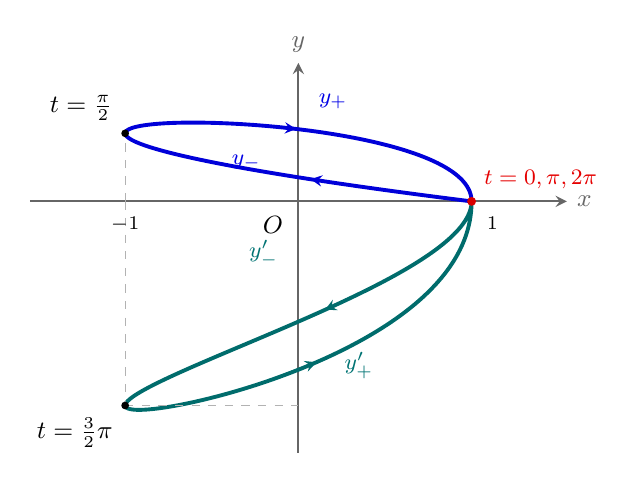
\begin{tikzpicture}[x=2.2cm, y=0.55cm, >=stealth, every node/.style={font=\small}]

    % --- 1. 座標軸 ---
    \draw[->, thick, gray!80!black] (-1.55, 0) -- (1.55, 0) node[right] {$x$};
    \draw[->, thick, gray!80!black] (0, -5.8) -- (0, 3.2) node[above] {$y$};
    \node[below left=2pt] at (0, 0) {$O$};

    % --- 2. 曲線 (x(t), y(t)) の描画 (trig format=rad で安全に計算) ---
    % 上側ループ: 0 <= t <= pi
    \draw[line width=1.4pt, blue!85!black, domain=0:3.14159, samples=80, smooth, variable=\t, trig format=rad]
    plot ({cos(2*\t)}, {\t*sin(\t)});

    % 下側ループ: pi <= t <= 2*pi
    \draw[line width=1.4pt, teal!85!black, domain=3.14159:6.28319, samples=90, smooth, variable=\t, trig format=rad]
    plot ({cos(2*\t)}, {\t*sin(\t)});

    % --- 3. 進行方向の矢印 (明示的な座標指定でオーバーフローを完全回避) ---
    % 上側ループの矢印 (t ≈ 0.6, t ≈ 2.2)
    \draw[->, thick, blue!85!black]
    ({cos(2*0.6 r)}, {0.6*sin(0.6 r)}) -- ({cos(2*0.75 r)}, {0.75*sin(0.75 r)});
    \draw[->, thick, blue!85!black]
    ({cos(2*2.2 r)}, {2.2*sin(2.2 r)}) -- ({cos(2*2.35 r)}, {2.35*sin(2.35 r)});

    % 下側ループの矢印 (t ≈ 3.7, t ≈ 5.4)
    \draw[->, thick, teal!85!black]
    ({cos(2*3.7 r)}, {3.7*sin(3.7 r)}) -- ({cos(2*3.85 r)}, {3.85*sin(3.85 r)});
    \draw[->, thick, teal!85!black]
    ({cos(2*5.4 r)}, {5.4*sin(5.4 r)}) -- ({cos(2*5.55 r)}, {5.55*sin(5.55 r)});

    % --- 4. 特徴点・補助線 ---
    % t = pi/2: (-1, pi/2)
    \coordinate (P_top) at (-1, 1.5708);
    \draw[dashed, gray!60] (-1, 0) -- (P_top);
    \fill[black] (P_top) circle (1.4pt) node[above left=1pt] {$t = \frac{\pi}{2}$};

    % t = 3pi/2: (-1, -3pi/2)
    \coordinate (P_bot) at (-1, -4.7124);
    \draw[dashed, gray!60] (-1, 0) -- (P_bot);
    \draw[dashed, gray!60] (P_bot) -- (0, -4.7124);
    \fill[black] (P_bot) circle (1.4pt) node[below left=1pt] {$t = \frac{3}{2}\pi$};

    % x = -1, 1 の目盛り
    \node[below=2pt, font=\scriptsize] at (-1, 0) {$-1$};
    \node[below right=2pt, font=\scriptsize] at (1, 0) {$1$};

    % 3重交点 (1, 0)
    \coordinate (P_cross) at (1, 0);
    \fill[red!85!black] (P_cross) circle (1.6pt);
    \node[above right=1pt, font=\footnotesize\bfseries, red!90!black] at (P_cross) {$t = 0, \pi, 2\pi$};

    % --- 5. 枝ラベル (y_+, y_-, y'_-, y'_+) ---
    \node[blue!90!black, font=\footnotesize\bfseries] at (0.2, 2.3) {$y_+$};
    \node[blue!90!black, font=\footnotesize\bfseries] at (-0.3, 0.9) {$y_-$};
    \node[teal!90!black, font=\footnotesize\bfseries] at (-0.2, -1.2) {$y'_-$};
    \node[teal!90!black, font=\footnotesize\bfseries] at (0.35, -3.8) {$y'_+$};

  \end{tikzpicture}
  \caption{曲線 $(x, y) = (\cos 2t, t\sin t)$ の概形と各枝の対応関係}
  \label{fig:parametric_curve_loops_fixed}
\end{figure}

そこで求める面積$S$のうち，$y\ge0$に含まれるものを$S_1$，$y\le0$に含まれるものを$S_2$とすると，
\begin{align}
  S=S_1+S_2 \label{eq:5}
\end{align}
である．それぞれを計算すると
\begin{align}
  S_1= \int_{-1}^{1}(y_{+}-y_{-})dx
  = \int_{\pi/2}^{\pi}y_{+}\dfrac{dx}{dt}dt - \int_{\pi/2}^{0}y_{-}\dfrac{dx}{dt}dt
  = \int_{0}^{\pi}y\dfrac{dx}{dt}
  = \int_0^\pi g(t)f'(t)\,dt \label{eq:6}
\end{align}
および
\begin{align}
  S_2= \int_{-1}^{1}(y'_{-}-y'_{+})dx
  = \int_{3\pi/2}^{\pi}y'_{-}\dfrac{dx}{dt}dt - \int_{3\pi/2}^{2\pi}y'OB_{+}\dfrac{dx}{dt}dt
  = -\int_{\pi}^{2\pi} g(t)f'(t)\,dt \label{eq:7}
\end{align}
である．ここで\cref{eq:1}よりこれらの被積分関数は
\begin{align}
  g(t)f'(t)
  &=t\sin t (-4\sin t\cos t)
  =-4t\cos t(1-\cos^2t)
  =-4t(\cos t-\cos^3t) \\
  &=-4t\left[\cos t - \dfrac{3\cos t+\cos 3t}{4}\right]
  =-t\cos t + t\cos 3t
\end{align}
だから不定積分は積分定数を抜いて
\begin{align}
  \int g(t)f'(t)\,dt
  &=-\int t\cos t\,dt+\int t\cos 3t\,dt\\
  &=-(t\sin t+\cos t)+\left(\dfrac{1}{3}t\sin 3t + \dfrac{1}{9}\cos 3t\right) \equiv F(t)
\end{align}
である．よって
\begin{align}
  F(0)  &=-1+\dfrac{1}{9}=-\dfrac{8}{9} \\
  F(\pi)&=1-\dfrac{1}{9}=\dfrac{8}{9} \\
  F(2\pi)&=-1+\dfrac{1}{9}=-\dfrac{8}{9}
\end{align}
だから，\cref{eq:6,eq:7}より
\begin{align}
  S_1&=F(\pi)-F(0)=\dfrac{8}{9}-\left(-\dfrac{8}{9}\right)=\dfrac{16}{9}\\
  S_2&=-\{F(2\pi)-F(\pi)\}=-\left(-\dfrac{8}{9}-\dfrac{8}{9}\right)=\dfrac{16}{9}
\end{align}
となって，\cref{eq:5}に代入して
\begin{align}
  S=\dfrac{16}{9}+\dfrac{16}{9}=\dfrac{32}{9}
\end{align}
である．

\end{document}
